\documentclass[12pt]{article}[margin=1in]
\usepackage{fullpage,graphicx,psfrag,amsmath,amsfonts,verbatim}
\usepackage{multicol,multirow}
\usepackage[small,bf]{caption}
\usepackage{amsthm}
\usepackage{hyperref}
\usepackage{bbm} % for the indicator function to look good
\usepackage{color}
\usepackage{mathtools}
\usepackage{fancyhdr} % for the header
\usepackage{booktabs} % for regression table display (toprule, midrule, bottomrule)
\usepackage{adjustbox} % for regression table display
\usepackage{threeparttable} % to use table notes
\usepackage{natbib} % for bibliography
\input newcommand.tex
\bibliographystyle{apalike}
\setlength{\parindent}{0pt} \renewcommand{\thesection}{Question \arabic{section}}
\renewcommand{\thesubsection}{\arabic{section}.\arabic{subsection}}% remove the automatic indentation % for problem set

% Settings for page number in the footer
\pagestyle{fancy}
\fancyhf{}
\fancyfoot[C]{\thepage}
\renewcommand{\headrulewidth}{0pt}
\renewcommand{\footrulewidth}{0pt}

\title{\textbf{Estimate Dynamic Models with CCP} \\
    \vspace{.3cm}
    \large Problem Set 1 \\
    Empirical Industrial Organization 2025 Srping}
\author{Zixuan}
\date{\today}

\begin{document}
\maketitle

\setcounter{page}{1}

\paragraph{Utility (Profit)}
The profit function of the Harold Zurcher is
\begin{equation*}
    u(s,Y) = (-RC)Y + (-\mu s)(1 - Y) = (-RC + \mu s)Y - \mu s
\end{equation*}
The realized profit is
\begin{equation*}
    v(s,Y,\nu_0,\nu_1) = u(s,Y) + \nu_Y
\end{equation*}

\paragraph{Variables} For \textbf{observed variables}, we have
\begin{itemize}
    \item $s$: the state variable, the mileage at the end of period $t$
    \item $Y$: the decision variable, the decision to replace the bus at the end of period $t$
\end{itemize}
For \textbf{unobserved variables}, we have $\nu_0,\nu_1$.
\paragraph{State transition} The state variable $s$ evolves according to this transition function
\begin{equation*}
    s_{t+1} = s_t + \epsilon_{t+1} \quad \epsilon_{t+1} \sim N(\rho, \sigma_{\rho}^2)
\end{equation*}
\paragraph{Parameters} The profit function parameters:
\begin{itemize}
    \item $\mu$: the cost of maintaining the bus
    \item $RC$: the replacement cost of the bus
\end{itemize}
The state transition parameters: $\rho$ and $\sigma_{\rho}^2$.
Discount factor $\beta=0.99$ is given.

\paragraph{Value function} The value function is
\begin{equation*}
    \begin{split}
        V(s, \nu) & = \max_{Y} \left\{ v(s,Y,\nu) + \beta \mathbb{E}[V(s', \nu')|s,Y] \right\}                       \\
                  & = \max_{Y} \left\{ u(s,Y)+\nu_Y + \beta \int \mathbb{E}_{\nu'}[V(s', \nu')] f(s'|s) ds' \right\} \\
    \end{split}
\end{equation*}

To understand this value function, notice that at the end of each period $t$
Harold Zurcher is essentially comparing the \textbf{continuation value} from
replacing $Y=1$ and that from not replacing $Y=0$. We define the
\textbf{continuation value} as $\tilde{v}(s,Y,\nu)$. The value function is the
maximum of them.
\begin{align*}
    \tilde{v}(s,1,\nu) & = \tilde{u}(s,1) + \nu_1=  (-RC + \mu s) +\nu_1 + \beta \int \mathbb{E}_{\nu'}[V(s', \nu')|s,1] f(s'|s) ds' \\
    \tilde{v}(s,0,\nu) & = \tilde{u}(s,0)+\nu_0 = \nu_0+\beta \int \mathbb{E}_{\nu'}[V(s', \nu')|s,0] f(s'|s) ds'
\end{align*}
Therefore the value function can be rewritten as
\begin{equation*}
    V(s, \nu) = \max_Y\left\{ \tilde{v}(s,1,\nu), \tilde{v}(s,0,\nu) \right\}
\end{equation*}

If we know the $\tilde{u}(s,1)$ and $\tilde{u}(s,0)$, and assume $\nu$ are iid
from T1EV, we are back to the static logit discrete choice model such that
\begin{equation*}
    \Pr(Y=1|s) = \frac{\exp(\tilde{u}(s,1))}{\exp(\tilde{u}(s,1)) + \exp(\tilde{u}(s,0))}
\end{equation*}

We follow \citet{bajari2007estimating} to approximate the continuation value
$\tilde{v}$ by
\begin{align*}
    \tilde{v}(s,1,\nu) & = \tilde{u}(s,1) + \nu_1 = x_{i1}^1\ + x_{i1}^2\beta_2 + x_{i1}^3+ \nu_1     \\
    \tilde{v}(s,0,\nu) & = \tilde{u}(s,0) +\nu_0 = x_{i0}^1\beta_1 + x_{i0}^2\beta_2 + x_{i0}^3+\nu_0
\end{align*}
Where
\begin{itemize}
    \item $x_{i}^1 = -\frac{1}{K}\sum_{k=1}^K \sum_{t=1}^T Y_{it}$
    \item $x_{i}^2 = -\frac{1}{K}\sum_{k=1}^K \sum_{t=1}^T s_{it}(1-Y_{it})$
    \item $x_{i}^3 = \frac{1}{K}\sum_{k=1}^K \sum_{t=1}^T (\gamma-\ln(\Pr(Y_{it}|s_{it})))$: \textbf{I was tripped by this term.} It is $\ln(\Pr(Y=1|s))$ when $Y_{it}=1$ and $\ln(\Pr(Y=0|s))$ when $Y_{it}=0$.
\end{itemize}
Therefore, we obtain $RC=\beta_1, \mu=\beta_2$.

The optimal $\theta^*$ is the one that maximizes the likelihood function
\begin{equation}\label{eq:likelihood}
    \max_{\theta} \sum_{i=1}^N \sum_{t=1}^T \ln \Pr(Y_{it}|s_{it},\theta)
\end{equation}

\section{Reduced Form CCP (Probit)}

Estimating a reduced form conditional choice probability is the preparation
step for simulation. Experimenting with 4 different specifications.
\begin{itemize}
    \item \verb|probit1|: $\Pr(Y=1|s) = \Phi(\gamma_0 + \gamma_1 s)$
    \item \verb|probit2|: $\Pr(Y=1|s) = \Phi(\gamma_0 + \gamma_1 s + \gamma_2 s^2)$
    \item \verb|probit3|: $\Pr(Y=1|s) = \Phi(\gamma_0 + \gamma_1 s + \gamma_2 s^2 + \gamma_3 s^3)$
    \item \verb|probitlog|: $\Pr(Y=1|s) = \Phi(\gamma_0 + \gamma_1 \ln(s))$
\end{itemize}
Then, we plot the estimated CCPs against a range of value for $s\in[0,40]$. Results are shown in Figure~\ref{fig:ccp_probit}. I chose the \verb|probit1| for later simulation.
\begin{figure}[!htbp]
    \centering
    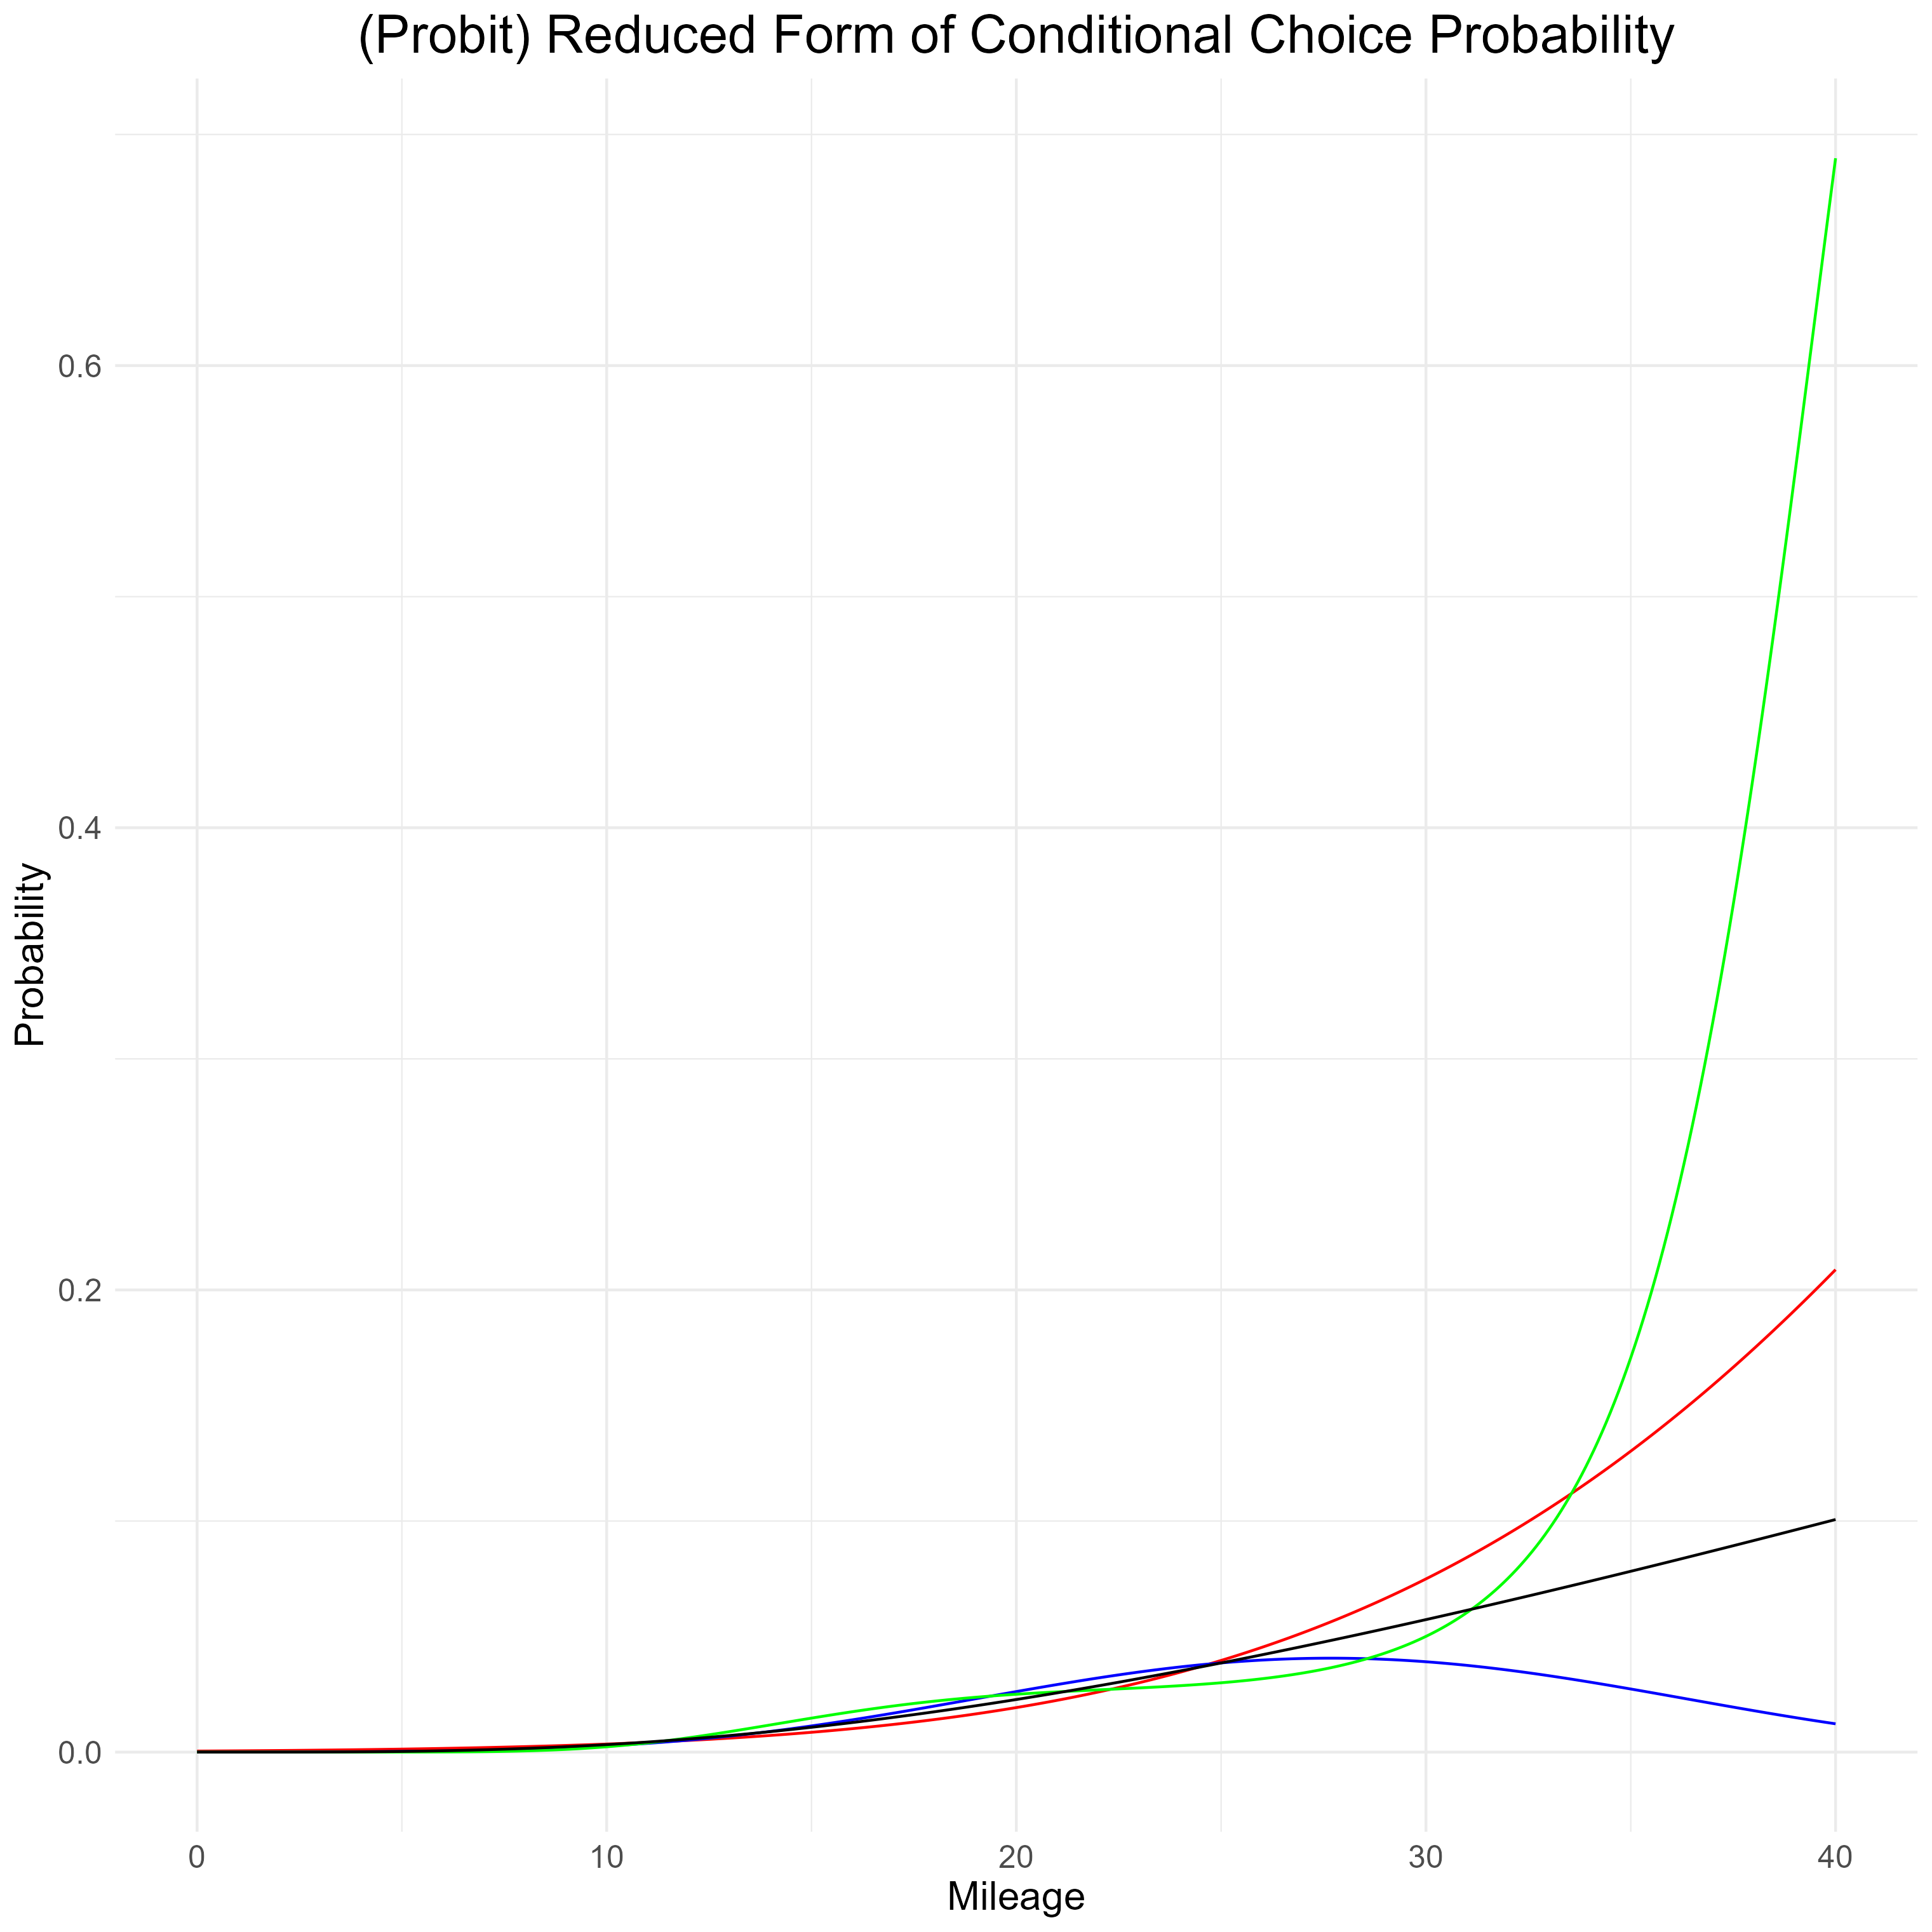
\includegraphics[width=0.6\textwidth]{../Figures/ccp_probit.png}
    \caption{Estimated Reduced Form CCPs from Probit Models}
    \label{fig:ccp_probit}
\end{figure}

\section{State Transition}
The transition of states is guided by $\epsilon\in N(\rho, \sigma_{\rho}^2)$.
This is a somewhat unrealistic assumption since the mileage can only increase.
However, we proceed as instructed.
\begin{itemize}
    \item $\rho=0.19$
    \item $\sigma_{\rho}^2=0.0129$
\end{itemize}

\section{Simulation}\label{sec:simulation}
For each observation $\text{bus} \times \text{period}$, we perform simulation
to get the 6 variables $x_{i1}^1,x_{i1}^2,x_{i1}^3$ and
$x_{i0}^1,x_{i0}^2,x_{i0}^3$. Then, we take average over all observations to
get Table~\ref{tab:sim_avg}.

\begin{table}[!htbp]
    \centering
    % latex table generated in R 4.3.1 by xtable 1.8-4 package
% Mon Feb  3 22:53:54 2025
\begin{tabular}{rrr}
  \hline
          & Replace & Non Replace \\
  \hline
  $x_i^1$ & -1.19   & -0.57       \\
  $x_i^2$ & -436.09 & -702.38     \\
  $x_i^3$ & 37.81   & 39.42       \\
  \hline
\end{tabular}

    \caption{Average of Simulation Results}
    \label{tab:sim_avg}
\end{table}

\section{Estimation}\label{sec:estimation}
We estimate by Equation~\ref{eq:likelihood} using the simulated approximation.
Results are shown in Table~\ref{tab:est_results}.
\begin{table}[!htbp]
    \centering
    
% Table created by stargazer v.5.2.3 by Marek Hlavac, Social Policy Institute. E-mail: marek.hlavac at gmail.com
% Date and time: Tue, Feb 04, 2025 - 2:32:08 pm
\begin{tabular}{@{\extracolsep{5pt}}lc} 
\\[-1.8ex]\hline 
\hline \\[-1.8ex] 
 & \multicolumn{1}{c}{\textit{Dependent variable:}} \\ 
\cline{2-2} 
\\[-1.8ex] & choice \\ 
\hline \\[-1.8ex] 
 RC & 8.795$^{***}$ \\ 
  & (0.733) \\ 
  & \\ 
 $\mu$ & 0.005$^{***}$ \\ 
  & (0.001) \\ 
  & \\ 
\hline \\[-1.8ex] 
Observations & 7,250 \\ 
Log Likelihood & $-$319.716 \\ 
Akaike Inf. Crit. & 643.432 \\ 
\hline 
\hline \\[-1.8ex] 
\textit{Note:}  & \multicolumn{1}{r}{$^{*}$p$<$0.1; $^{**}$p$<$0.05; $^{***}$p$<$0.01} \\ 
\end{tabular} 

    \caption{Estimation Results}
    \label{tab:est_results}
\end{table}

\section{Comparison}

In order to plot the CCPs estimated from ~\ref{sec:estimation} against mileage
$s$, we first simulate for each $s\in [0,40]$ exactly as in
~\ref{sec:simulation}. Then we use the estimated parameters $\theta^*$ to
compute the CCPs. The results are shown in Figure~\ref{fig:ccp_dynamic}.
Alternatively, one could take the parameters $\theta^*$ and solve the dynamic
programming problem analytically as in \citet{rust1987optimal}. Solving for
$\bar{V}(s)$ from Equation~\ref{eq:exp_v} and then compute CCP from
Equation~\ref{eq:ccp}.

\begin{align}
    \bar{V}(s) & =\gamma+\ln\left(\sum_{Y} \exp\left(u(s,Y)+\beta\int \bar{V}(s') f(s'|s) ds'\right)\right)                                        \label{eq:exp_v}                                     \\
    \Pr(Y=1|s) & =\frac{\exp\left\{ u(s,Y=1) + \beta \sum_{s'}\bar{V}(s') \Pr(s'|s,Y)\right\}}{\sum_{Y \in \{0,1\}} \exp\left\{ u(s,Y) + \beta \sum_{s'}\bar{V}(s') \Pr(s'|s,Y)\right\}} \label{eq:ccp}
\end{align}

\begin{figure}
    \centering
    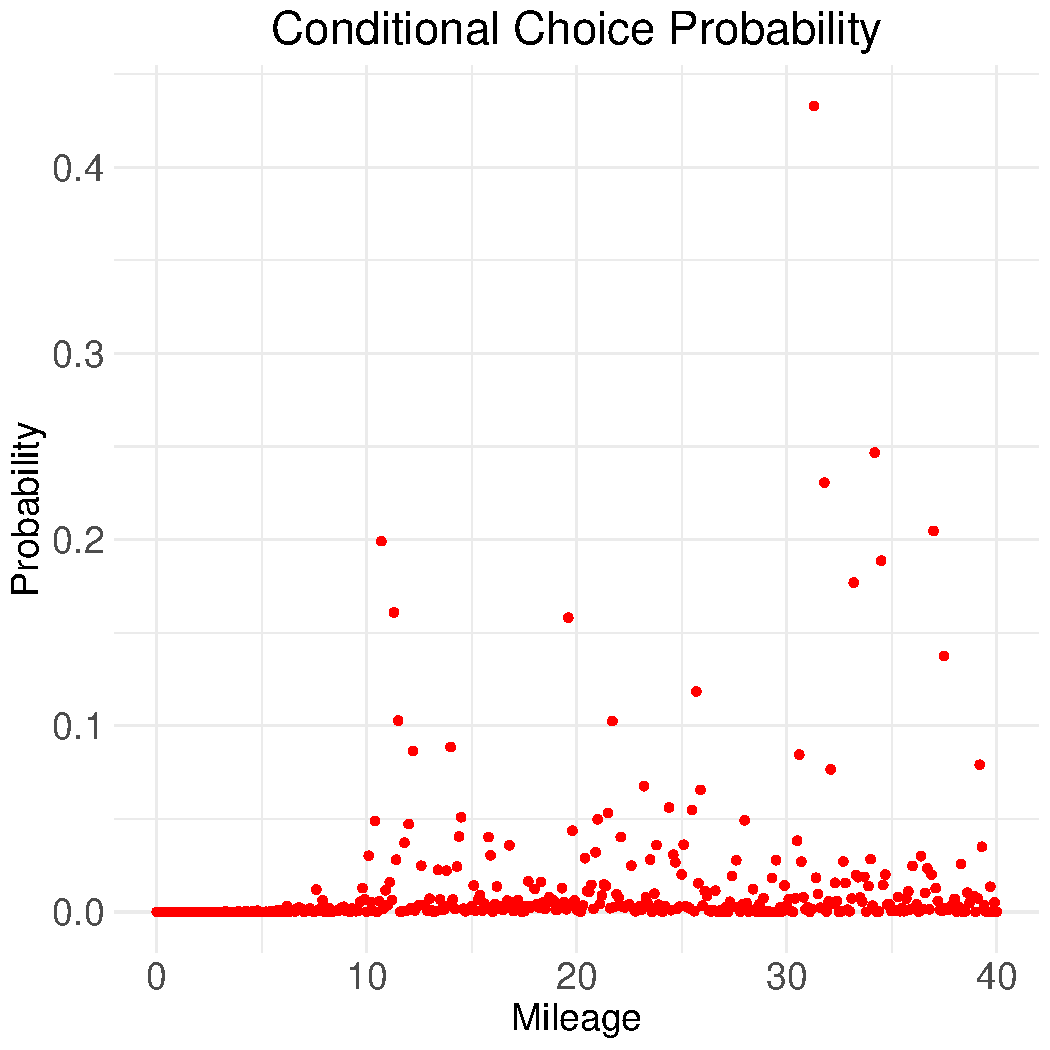
\includegraphics[width=0.6\textwidth]{../Figures/ccp_dynamic.pdf}
    \caption{Estimated dynamic CCPs following \citet{bajari2007estimating}.}
    \label{fig:ccp_dynamic}
\end{figure}

% \paragraph{Expected value function} We define the expected value function as
% \begin{equation*}
%     \bar{V}(s)=\int \max_{Y} \left\{ u(s,Y)+\nu_Y + \beta \int \mathbb{E}_{\nu'}[V(s', \nu')] f(s') ds' \right\} f(\nu_0,\nu_1) d(\nu_0,\nu_1)
% \end{equation*}
% From the property of $\nu_0,\nu_1$ as well as $\nu_0-\nu_1$ from T1EV, we have
% \begin{equation*}\label{eq:full}
%     \bar{V}(s)=\gamma+\ln\left(\sum_{Y} \exp\left(u(s,Y)+\beta\int \bar{V}(s') f(s'|s) ds'\right)\right)
% \end{equation*}
% Recall what we do in the CCP estimation algorithm, we would rewrite Equation~\ref{eq:full} as
% \begin{equation*}\label{eq:ccp}
%     \bar{V}(s)=\sum_{Y\in\set{0,1}} \Pr(Y|s) \left(u(s,Y)+\mathbb{E}_{\nu_Y}[\nu_Y|s, Y]+ \beta \int \bar{V}(s') f(s'|s) ds'\right)
% \end{equation*}
% Replacing $\mathbb{E}_{\nu_Y}[\nu_Y|s, Y]$ with $\gamma_Y-\ln\Pr(Y|s)$, we have
% \begin{equation*}
%     \begin{split}
%         \bar{V}(s)&=\gamma+\Pr(Y=0|s) \left(u(s,0)-\ln\Pr(Y=0|s)+ \beta \int \bar{V}(s') f(s'|s) ds'\right)\\
%         & +\Pr(Y=1|s) \left(u(s,1)-\ln\Pr(Y=1|s)+ \beta \int \bar{V}(s') f(s'|s) ds'\right)
%     \end{split}
% \end{equation*}

\bibliography{../References/ref.bib}

\end{document}